\documentclass[../main.tex]{subfiles}

\begin{figure}[ht]
    \centering
    \begin{subfigure}[b]{0.3\textwidth}
        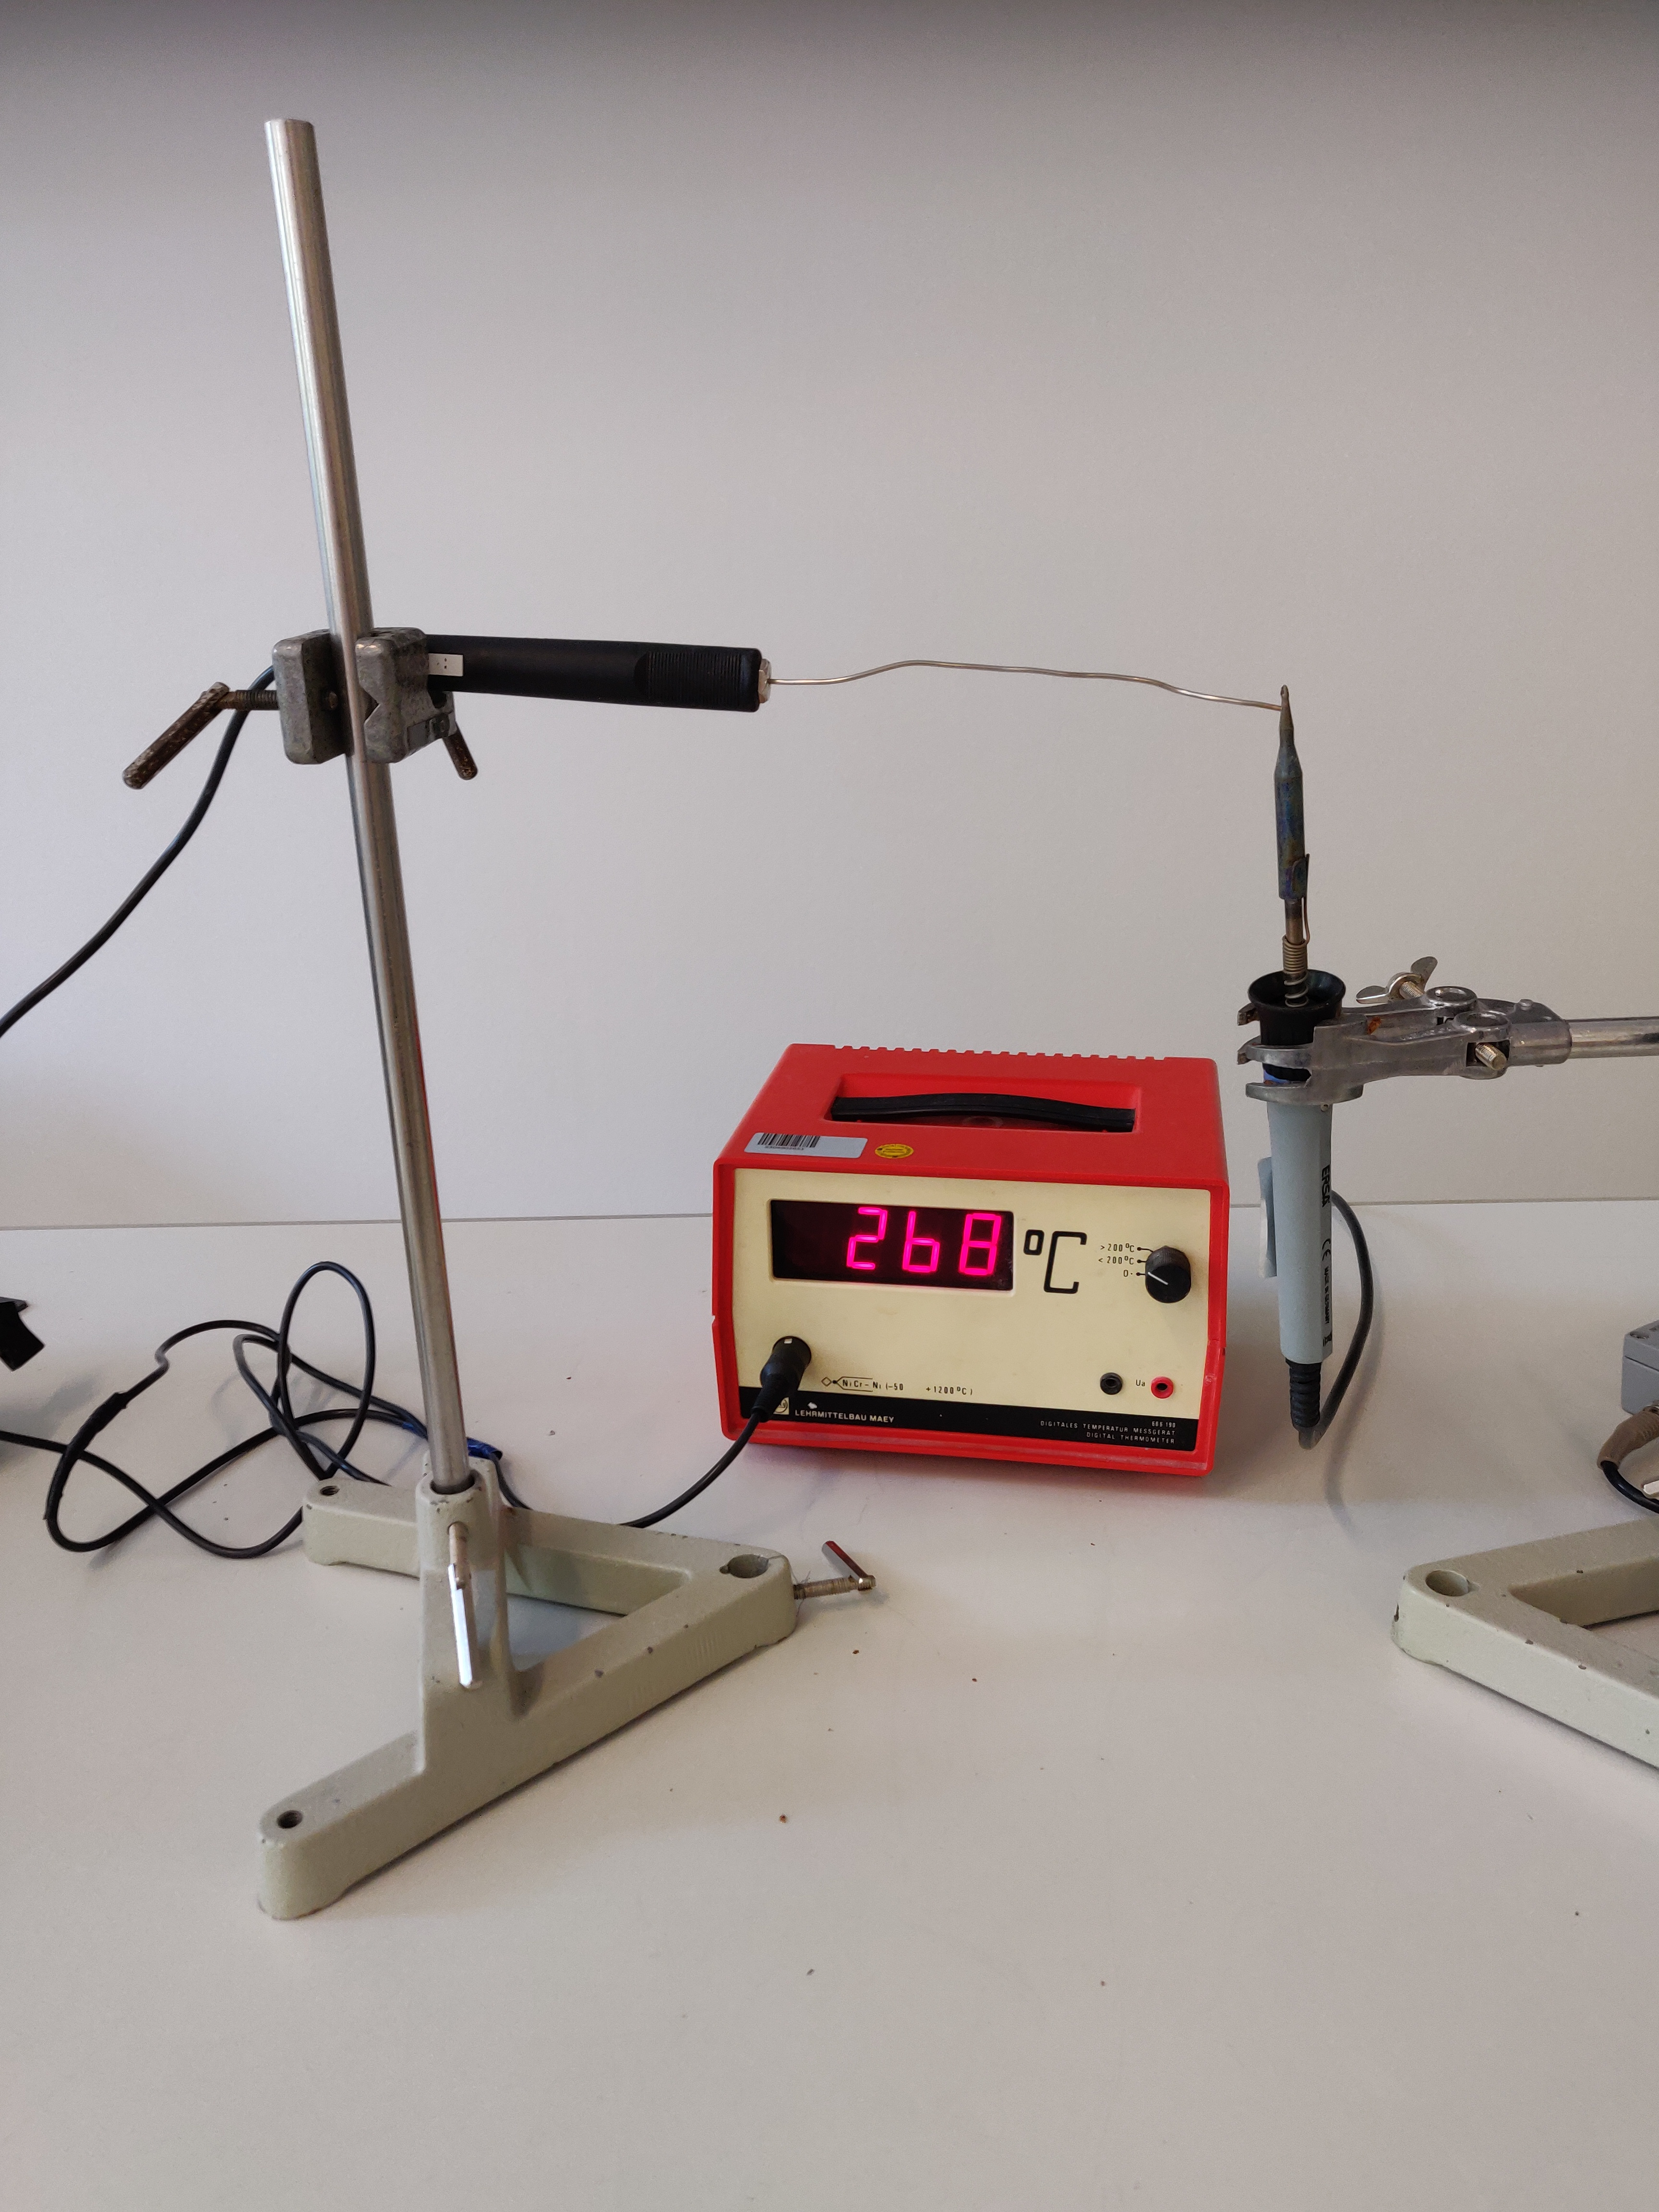
\includegraphics[width=\textwidth]{experiment/11-loetkolben-temperatur.jpg}
        \caption{Lötkolben}
        \label{fig:loetkolben}
    \end{subfigure}
    \begin{subfigure}[b]{0.3\textwidth}
        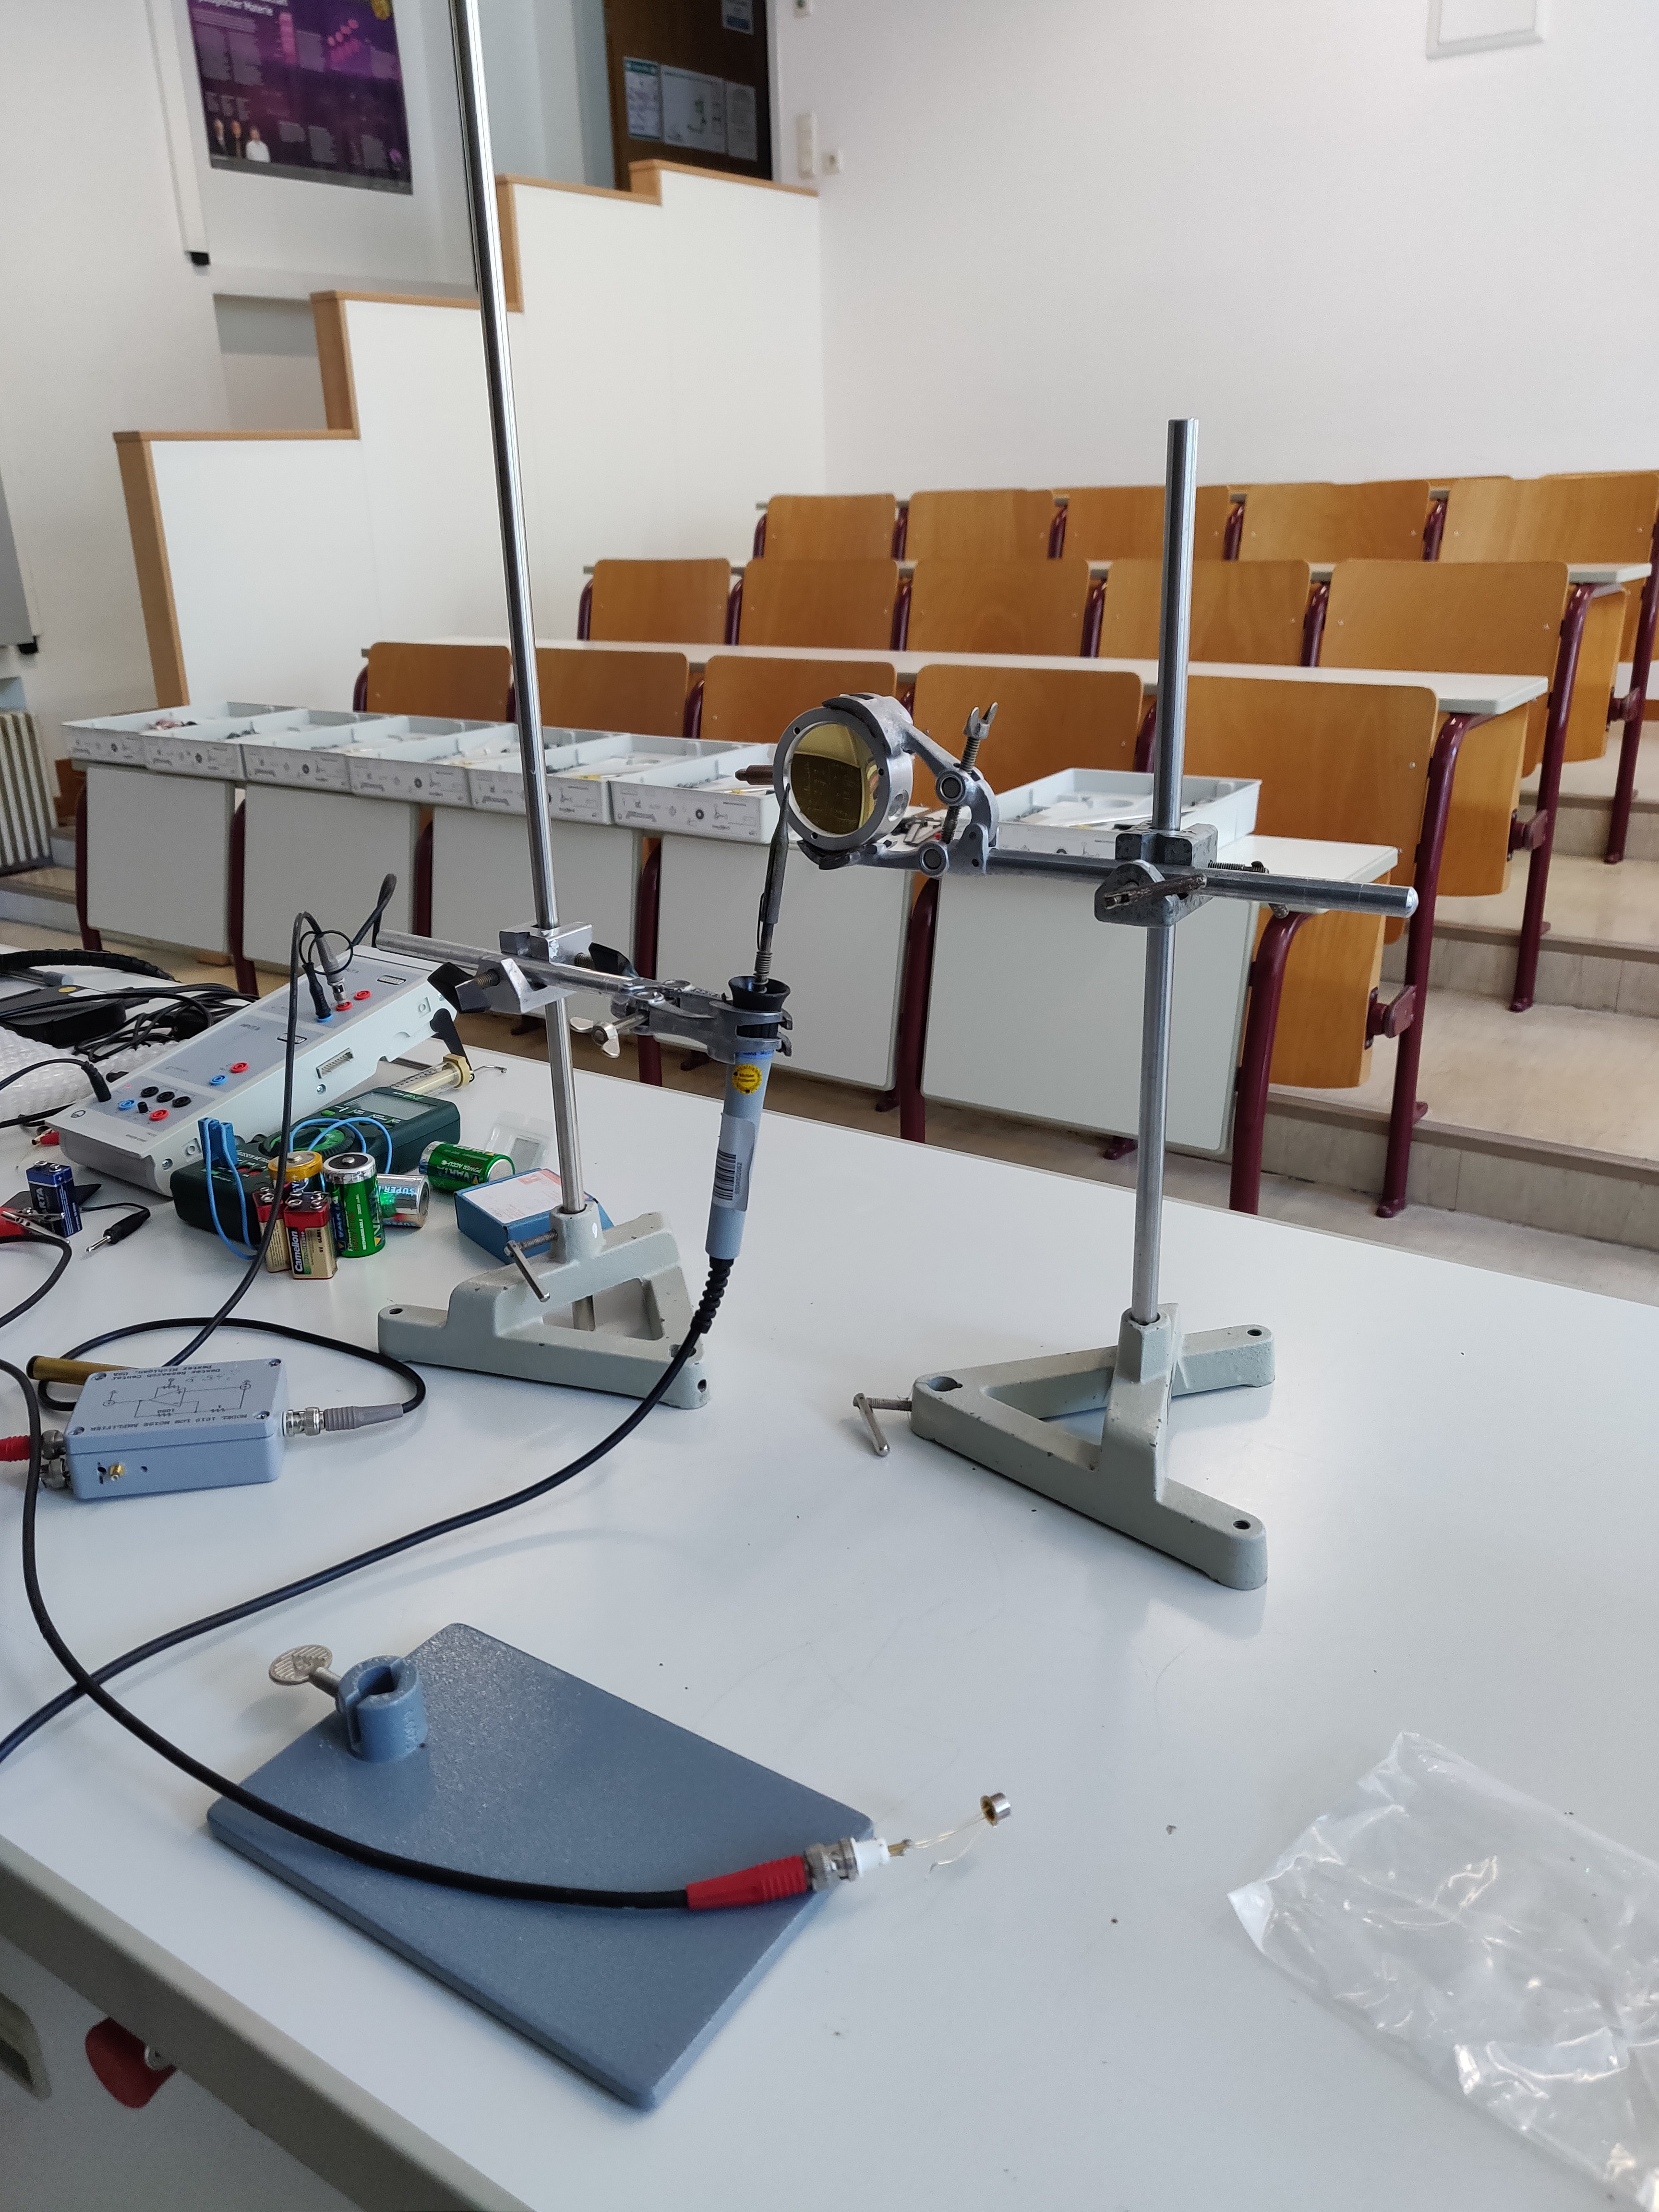
\includegraphics[width=\textwidth]{experiment/13-loetkolben-spiegel.jpg}
        \caption{Lötkolben mit Spiegel}
        \label{fig:loetkolben_mit_spiegel}
    \end{subfigure}
    \begin{subfigure}[b]{0.3\textwidth}
        \includegraphics[width=\textwidth]{experiment/29-leypold-gitter.jpg}
        \caption{Leybold Gitter}
        \label{fig:gitter_leybold}
    \end{subfigure}
    \caption{Notwendige Komponenten eines Spektrometers}
\end{figure}

Um ein IR-Spektrometer zu bauen, benötigen wir zunächst eine Strahlquelle im Infrarotbereich (Abb. \ref{fig:loetkolben}), einen Spiegel (Abb. \ref{fig:loetkolben_mit_spiegel}) zur reflexion auf das Gitter (Abb. \ref{fig:gitter_leybold}), welches die Strahlen beugt.

\subsubsection{Strahlquelle}
\subfile{3_1_1_strahlquelle.tex}

\subsubsection{Abbildende Optik}
\subfile{3_1_2_abbildende_optik}

\subsubsection{Optisches Gitter}
\subfile{3_1_3_optisches_gitter}
